% Plot mark gallery for npm run compare:renderers (every PGF mark, two sizes,
% fills, mark color and mark options).
\documentclass[tikz,border=2pt]{standalone}
\usetikzlibrary{plotmarks}
\begin{document}
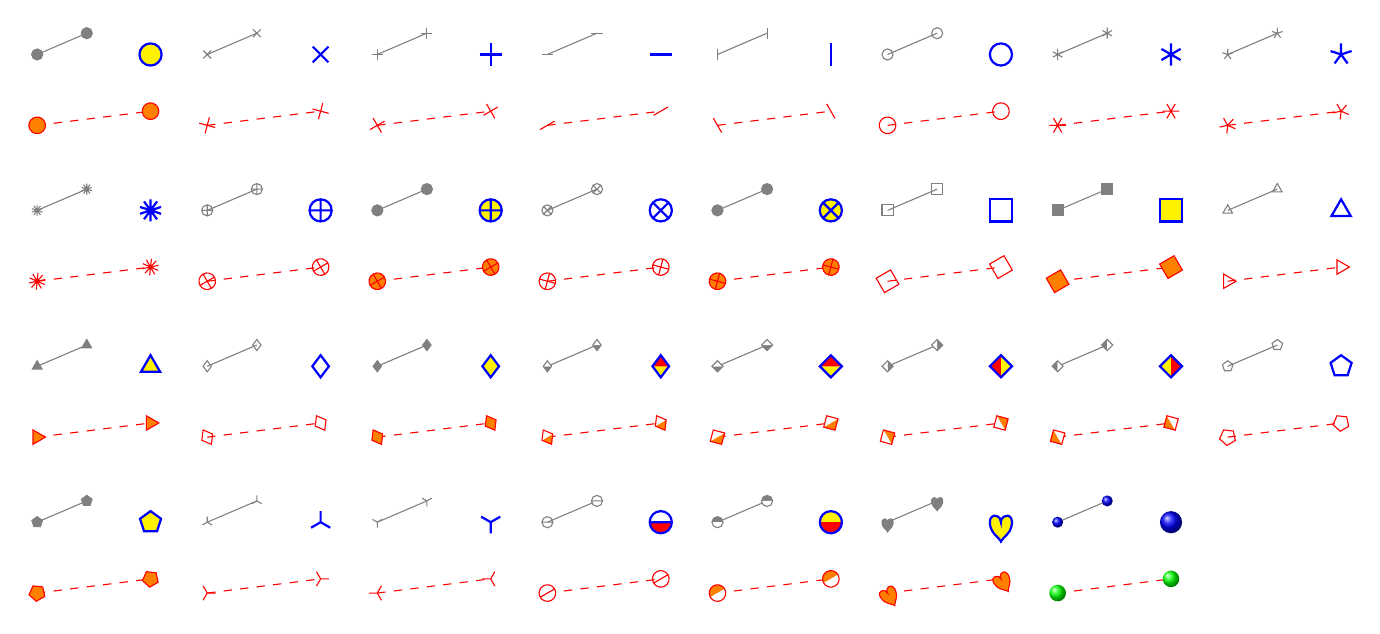
\begin{tikzpicture}[x=0.9cm,y=0.9cm]
  \draw[gray] plot[mark=*] coordinates {(0,0) (0.7,0.3)};
  \draw[draw=blue, fill=yellow, mark color=red, thick] plot[only marks, mark=*, mark size=4pt] coordinates {(1.6,0)};
  \draw[red, dashed] plot[mark=*, mark size=3pt, mark options={solid, rotate=30, fill=orange, ball color=green}] coordinates {(0,-1.0) (1.6,-0.8)};
  \draw[gray] plot[mark=x] coordinates {(2.4,0) (3.1,0.3)};
  \draw[draw=blue, fill=yellow, mark color=red, thick] plot[only marks, mark=x, mark size=4pt] coordinates {(4.0,0)};
  \draw[red, dashed] plot[mark=x, mark size=3pt, mark options={solid, rotate=30, fill=orange, ball color=green}] coordinates {(2.4,-1.0) (4.0,-0.8)};
  \draw[gray] plot[mark=+] coordinates {(4.8,0) (5.5,0.3)};
  \draw[draw=blue, fill=yellow, mark color=red, thick] plot[only marks, mark=+, mark size=4pt] coordinates {(6.4,0)};
  \draw[red, dashed] plot[mark=+, mark size=3pt, mark options={solid, rotate=30, fill=orange, ball color=green}] coordinates {(4.8,-1.0) (6.4,-0.8)};
  \draw[gray] plot[mark=-] coordinates {(7.199999999999999,0) (7.9,0.3)};
  \draw[draw=blue, fill=yellow, mark color=red, thick] plot[only marks, mark=-, mark size=4pt] coordinates {(8.8,0)};
  \draw[red, dashed] plot[mark=-, mark size=3pt, mark options={solid, rotate=30, fill=orange, ball color=green}] coordinates {(7.199999999999999,-1.0) (8.8,-0.8)};
  \draw[gray] plot[mark=|] coordinates {(9.6,0) (10.3,0.3)};
  \draw[draw=blue, fill=yellow, mark color=red, thick] plot[only marks, mark=|, mark size=4pt] coordinates {(11.2,0)};
  \draw[red, dashed] plot[mark=|, mark size=3pt, mark options={solid, rotate=30, fill=orange, ball color=green}] coordinates {(9.6,-1.0) (11.2,-0.8)};
  \draw[gray] plot[mark=o] coordinates {(12,0) (12.7,0.3)};
  \draw[draw=blue, fill=yellow, mark color=red, thick] plot[only marks, mark=o, mark size=4pt] coordinates {(13.6,0)};
  \draw[red, dashed] plot[mark=o, mark size=3pt, mark options={solid, rotate=30, fill=orange, ball color=green}] coordinates {(12,-1.0) (13.6,-0.8)};
  \draw[gray] plot[mark=asterisk] coordinates {(14.399999999999999,0) (15.1,0.3)};
  \draw[draw=blue, fill=yellow, mark color=red, thick] plot[only marks, mark=asterisk, mark size=4pt] coordinates {(16.0,0)};
  \draw[red, dashed] plot[mark=asterisk, mark size=3pt, mark options={solid, rotate=30, fill=orange, ball color=green}] coordinates {(14.399999999999999,-1.0) (16.0,-0.8)};
  \draw[gray] plot[mark=star] coordinates {(16.8,0) (17.5,0.3)};
  \draw[draw=blue, fill=yellow, mark color=red, thick] plot[only marks, mark=star, mark size=4pt] coordinates {(18.4,0)};
  \draw[red, dashed] plot[mark=star, mark size=3pt, mark options={solid, rotate=30, fill=orange, ball color=green}] coordinates {(16.8,-1.0) (18.4,-0.8)};
  \draw[gray] plot[mark=10-pointed star] coordinates {(0,-2.2) (0.7,-1.9)};
  \draw[draw=blue, fill=yellow, mark color=red, thick] plot[only marks, mark=10-pointed star, mark size=4pt] coordinates {(1.6,-2.2)};
  \draw[red, dashed] plot[mark=10-pointed star, mark size=3pt, mark options={solid, rotate=30, fill=orange, ball color=green}] coordinates {(0,-3.2) (1.6,-3.0)};
  \draw[gray] plot[mark=oplus] coordinates {(2.4,-2.2) (3.1,-1.9)};
  \draw[draw=blue, fill=yellow, mark color=red, thick] plot[only marks, mark=oplus, mark size=4pt] coordinates {(4.0,-2.2)};
  \draw[red, dashed] plot[mark=oplus, mark size=3pt, mark options={solid, rotate=30, fill=orange, ball color=green}] coordinates {(2.4,-3.2) (4.0,-3.0)};
  \draw[gray] plot[mark=oplus*] coordinates {(4.8,-2.2) (5.5,-1.9)};
  \draw[draw=blue, fill=yellow, mark color=red, thick] plot[only marks, mark=oplus*, mark size=4pt] coordinates {(6.4,-2.2)};
  \draw[red, dashed] plot[mark=oplus*, mark size=3pt, mark options={solid, rotate=30, fill=orange, ball color=green}] coordinates {(4.8,-3.2) (6.4,-3.0)};
  \draw[gray] plot[mark=otimes] coordinates {(7.199999999999999,-2.2) (7.9,-1.9)};
  \draw[draw=blue, fill=yellow, mark color=red, thick] plot[only marks, mark=otimes, mark size=4pt] coordinates {(8.8,-2.2)};
  \draw[red, dashed] plot[mark=otimes, mark size=3pt, mark options={solid, rotate=30, fill=orange, ball color=green}] coordinates {(7.199999999999999,-3.2) (8.8,-3.0)};
  \draw[gray] plot[mark=otimes*] coordinates {(9.6,-2.2) (10.3,-1.9)};
  \draw[draw=blue, fill=yellow, mark color=red, thick] plot[only marks, mark=otimes*, mark size=4pt] coordinates {(11.2,-2.2)};
  \draw[red, dashed] plot[mark=otimes*, mark size=3pt, mark options={solid, rotate=30, fill=orange, ball color=green}] coordinates {(9.6,-3.2) (11.2,-3.0)};
  \draw[gray] plot[mark=square] coordinates {(12,-2.2) (12.7,-1.9)};
  \draw[draw=blue, fill=yellow, mark color=red, thick] plot[only marks, mark=square, mark size=4pt] coordinates {(13.6,-2.2)};
  \draw[red, dashed] plot[mark=square, mark size=3pt, mark options={solid, rotate=30, fill=orange, ball color=green}] coordinates {(12,-3.2) (13.6,-3.0)};
  \draw[gray] plot[mark=square*] coordinates {(14.399999999999999,-2.2) (15.1,-1.9)};
  \draw[draw=blue, fill=yellow, mark color=red, thick] plot[only marks, mark=square*, mark size=4pt] coordinates {(16.0,-2.2)};
  \draw[red, dashed] plot[mark=square*, mark size=3pt, mark options={solid, rotate=30, fill=orange, ball color=green}] coordinates {(14.399999999999999,-3.2) (16.0,-3.0)};
  \draw[gray] plot[mark=triangle] coordinates {(16.8,-2.2) (17.5,-1.9)};
  \draw[draw=blue, fill=yellow, mark color=red, thick] plot[only marks, mark=triangle, mark size=4pt] coordinates {(18.4,-2.2)};
  \draw[red, dashed] plot[mark=triangle, mark size=3pt, mark options={solid, rotate=30, fill=orange, ball color=green}] coordinates {(16.8,-3.2) (18.4,-3.0)};
  \draw[gray] plot[mark=triangle*] coordinates {(0,-4.4) (0.7,-4.1)};
  \draw[draw=blue, fill=yellow, mark color=red, thick] plot[only marks, mark=triangle*, mark size=4pt] coordinates {(1.6,-4.4)};
  \draw[red, dashed] plot[mark=triangle*, mark size=3pt, mark options={solid, rotate=30, fill=orange, ball color=green}] coordinates {(0,-5.4) (1.6,-5.2)};
  \draw[gray] plot[mark=diamond] coordinates {(2.4,-4.4) (3.1,-4.1)};
  \draw[draw=blue, fill=yellow, mark color=red, thick] plot[only marks, mark=diamond, mark size=4pt] coordinates {(4.0,-4.4)};
  \draw[red, dashed] plot[mark=diamond, mark size=3pt, mark options={solid, rotate=30, fill=orange, ball color=green}] coordinates {(2.4,-5.4) (4.0,-5.2)};
  \draw[gray] plot[mark=diamond*] coordinates {(4.8,-4.4) (5.5,-4.1)};
  \draw[draw=blue, fill=yellow, mark color=red, thick] plot[only marks, mark=diamond*, mark size=4pt] coordinates {(6.4,-4.4)};
  \draw[red, dashed] plot[mark=diamond*, mark size=3pt, mark options={solid, rotate=30, fill=orange, ball color=green}] coordinates {(4.8,-5.4) (6.4,-5.2)};
  \draw[gray] plot[mark=halfdiamond*] coordinates {(7.199999999999999,-4.4) (7.9,-4.1)};
  \draw[draw=blue, fill=yellow, mark color=red, thick] plot[only marks, mark=halfdiamond*, mark size=4pt] coordinates {(8.8,-4.4)};
  \draw[red, dashed] plot[mark=halfdiamond*, mark size=3pt, mark options={solid, rotate=30, fill=orange, ball color=green}] coordinates {(7.199999999999999,-5.4) (8.8,-5.2)};
  \draw[gray] plot[mark=halfsquare*] coordinates {(9.6,-4.4) (10.3,-4.1)};
  \draw[draw=blue, fill=yellow, mark color=red, thick] plot[only marks, mark=halfsquare*, mark size=4pt] coordinates {(11.2,-4.4)};
  \draw[red, dashed] plot[mark=halfsquare*, mark size=3pt, mark options={solid, rotate=30, fill=orange, ball color=green}] coordinates {(9.6,-5.4) (11.2,-5.2)};
  \draw[gray] plot[mark=halfsquare right*] coordinates {(12,-4.4) (12.7,-4.1)};
  \draw[draw=blue, fill=yellow, mark color=red, thick] plot[only marks, mark=halfsquare right*, mark size=4pt] coordinates {(13.6,-4.4)};
  \draw[red, dashed] plot[mark=halfsquare right*, mark size=3pt, mark options={solid, rotate=30, fill=orange, ball color=green}] coordinates {(12,-5.4) (13.6,-5.2)};
  \draw[gray] plot[mark=halfsquare left*] coordinates {(14.399999999999999,-4.4) (15.1,-4.1)};
  \draw[draw=blue, fill=yellow, mark color=red, thick] plot[only marks, mark=halfsquare left*, mark size=4pt] coordinates {(16.0,-4.4)};
  \draw[red, dashed] plot[mark=halfsquare left*, mark size=3pt, mark options={solid, rotate=30, fill=orange, ball color=green}] coordinates {(14.399999999999999,-5.4) (16.0,-5.2)};
  \draw[gray] plot[mark=pentagon] coordinates {(16.8,-4.4) (17.5,-4.1)};
  \draw[draw=blue, fill=yellow, mark color=red, thick] plot[only marks, mark=pentagon, mark size=4pt] coordinates {(18.4,-4.4)};
  \draw[red, dashed] plot[mark=pentagon, mark size=3pt, mark options={solid, rotate=30, fill=orange, ball color=green}] coordinates {(16.8,-5.4) (18.4,-5.2)};
  \draw[gray] plot[mark=pentagon*] coordinates {(0,-6.6000000000000005) (0.7,-6.3)};
  \draw[draw=blue, fill=yellow, mark color=red, thick] plot[only marks, mark=pentagon*, mark size=4pt] coordinates {(1.6,-6.6000000000000005)};
  \draw[red, dashed] plot[mark=pentagon*, mark size=3pt, mark options={solid, rotate=30, fill=orange, ball color=green}] coordinates {(0,-7.6) (1.6,-7.4)};
  \draw[gray] plot[mark=Mercedes star] coordinates {(2.4,-6.6000000000000005) (3.1,-6.3)};
  \draw[draw=blue, fill=yellow, mark color=red, thick] plot[only marks, mark=Mercedes star, mark size=4pt] coordinates {(4.0,-6.6000000000000005)};
  \draw[red, dashed] plot[mark=Mercedes star, mark size=3pt, mark options={solid, rotate=30, fill=orange, ball color=green}] coordinates {(2.4,-7.6) (4.0,-7.4)};
  \draw[gray] plot[mark=Mercedes star flipped] coordinates {(4.8,-6.6000000000000005) (5.5,-6.3)};
  \draw[draw=blue, fill=yellow, mark color=red, thick] plot[only marks, mark=Mercedes star flipped, mark size=4pt] coordinates {(6.4,-6.6000000000000005)};
  \draw[red, dashed] plot[mark=Mercedes star flipped, mark size=3pt, mark options={solid, rotate=30, fill=orange, ball color=green}] coordinates {(4.8,-7.6) (6.4,-7.4)};
  \draw[gray] plot[mark=halfcircle] coordinates {(7.199999999999999,-6.6000000000000005) (7.9,-6.3)};
  \draw[draw=blue, fill=yellow, mark color=red, thick] plot[only marks, mark=halfcircle, mark size=4pt] coordinates {(8.8,-6.6000000000000005)};
  \draw[red, dashed] plot[mark=halfcircle, mark size=3pt, mark options={solid, rotate=30, fill=orange, ball color=green}] coordinates {(7.199999999999999,-7.6) (8.8,-7.4)};
  \draw[gray] plot[mark=halfcircle*] coordinates {(9.6,-6.6000000000000005) (10.3,-6.3)};
  \draw[draw=blue, fill=yellow, mark color=red, thick] plot[only marks, mark=halfcircle*, mark size=4pt] coordinates {(11.2,-6.6000000000000005)};
  \draw[red, dashed] plot[mark=halfcircle*, mark size=3pt, mark options={solid, rotate=30, fill=orange, ball color=green}] coordinates {(9.6,-7.6) (11.2,-7.4)};
  \draw[gray] plot[mark=heart] coordinates {(12,-6.6000000000000005) (12.7,-6.3)};
  \draw[draw=blue, fill=yellow, mark color=red, thick] plot[only marks, mark=heart, mark size=4pt] coordinates {(13.6,-6.6000000000000005)};
  \draw[red, dashed] plot[mark=heart, mark size=3pt, mark options={solid, rotate=30, fill=orange, ball color=green}] coordinates {(12,-7.6) (13.6,-7.4)};
  \draw[gray] plot[mark=ball] coordinates {(14.399999999999999,-6.6000000000000005) (15.1,-6.3)};
  \draw[draw=blue, fill=yellow, mark color=red, thick] plot[only marks, mark=ball, mark size=4pt] coordinates {(16.0,-6.6000000000000005)};
  \draw[red, dashed] plot[mark=ball, mark size=3pt, mark options={solid, rotate=30, fill=orange, ball color=green}] coordinates {(14.399999999999999,-7.6) (16.0,-7.4)};
\end{tikzpicture}
\end{document}
